\documentclass[12pt,a4paper]{article}

\usepackage[utf8]{inputenc}
\usepackage[a4paper,total={150mm,240mm}]{geometry}
\usepackage[american]{babel}

\usepackage{float}
\usepackage{babel}
\usepackage{amsmath}
\usepackage{tikz}
\usepackage{graphicx}
\usepackage{amssymb}

\usepackage{listings}
\definecolor{listingbg}{gray}{0.95}
\lstset{language=C++,basicstyle=\ttfamily\small,frame=single,backgroundcolor=\color{listingbg}}
% \lstset{language=C++, basicstyle=\ttfamily,
%   keywordstyle=\color{black}\bfseries, tabsize=4, stringstyle=\ttfamily,
%   commentstyle=\it, extendedchars=true, escapeinside={/*@}{@*/}}

\usepackage{exercise}

\newcommand{\vx}{\vec x}
\newcommand{\uu}{\textbf u}
\newcommand{\nn}{\textbf n}
\newcommand{\grad}{\vec \nabla}
\newcommand{\wind}{\vec \beta}
\newcommand{\Laplace}{\Delta}


\title{\textbf{Exercises for the introduction to the Grid Interface}}
\exerciselabel{Exercise}

\begin{document}

\exerciseheader

\begin{Exercise}{Iterating over a grid}

First, you should start a fresh terminal and switch to the working directory of this exercise:
\begin{lstlisting}
  [user@dune-vm ~]$ cd dune-course
  [user@dune-vm dune-course]$ cd release-build
  [user@dune-vm release-build]$ cd dune-pdelab-tutorials
  [user@dune-vm dune-pdelab-tutorials]$ cd gridinterface
  [user@dune-vm gridinterface]$ cd exercise
  [user@dune-vm exercise]$ cd task
\end{lstlisting}

This is the build directory, so typing \lstinline!make! will build three executables.
To switch to the source directory, where the actual \lstinline!.cc! files are located, type \lstinline!cd src_dir!.
To switch back to the build directory, type \lstinline!cd ..!.

Open the file \texttt{grid-exercise1.cc} in a text editor.  It is an
example code that creates a structured grid (using the DUNE class
\texttt{YaspGrid}). The printgrid function then visualizes the grid
as a png file with some useful information, like global and local
indices, boundary intersections and such. You can have a look at the
visualization after a succesful run of the executable \lstinline!grid-exercise1!
with:

\begin{lstlisting}
  [user@dune-vm task]$ xdg-open printgrid_0.png
\end{lstlisting}%$

By default, a 4x4 grid is generated. You can change this to some
other number, recompile and rerun the executable and have a look at
the new grid visualization.

The code then iterates over all elements of this grid and
over all intersections of each element.  The code is meant to print
some information about the grid cells and the intersections (but it
does not yet).  The file is intermingled by suggestions what to print.
You are invited to follow these suggestions or to try any of the
member functions you learned about in the lectures.

\begin{center}
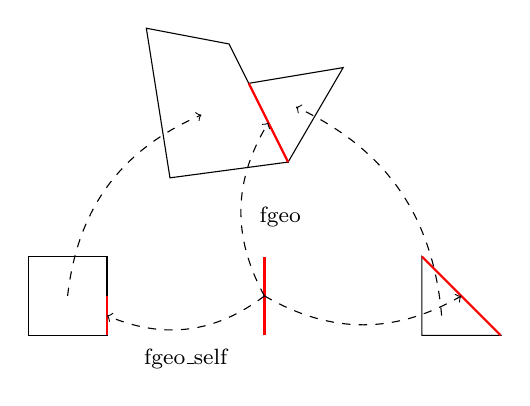
\begin{tikzpicture}[font=\footnotesize, scale=1.0]
  % Reference elements
  \draw (0,0) rectangle (1,1);
  \draw (5,0) -- (6,0) -- (5,1) -- cycle;

  % Reference intersection
  \draw (3,0) -- (3,1);

  % Elements
  \draw (3.3,2.2) -- (2.55,3.7) -- (1.5,3.9) -- (1.8,2.0) -- cycle;
  \draw (3.3,2.2) -- (2.8,3.2) -- (4.0,3.4) -- cycle;

  % Mark inersection in red
  \draw[thick,red] (3,0) -- (3,1);
  \draw[thick,red] (1,0) -- (1,0.5);
  \draw[thick,red] (5,1) -- (6,0);
  \draw[thick,red] (3.3,2.2) -- (2.8,3.2);

   % Coordinates for drawing dashed arrows
   %
   % r -> reference
   % w -> world
   \path
   (3.0,0.5) coordinate(ir)
   (1,0.25) coordinate(ie1r)
   (5.5,0.5) coordinate(ie2r)
   (3.05,2.7) coordinate(iw)
   (0.5,0.5) coordinate(e1r)
   (5.25,0.25) coordinate(e2r)
   (2.2,2.8) coordinate(e1w)
   (3.4,2.9) coordinate(e2w);

   % Draw dashed arrows for mappings
   \draw[dashed] (ir) edge[->,bend left] (iw);
   \draw[dashed] (ir) edge[->,bend left] (ie1r);
   \draw[dashed] (ir) edge[->,bend right] (ie2r);
   \draw[dashed] (e1r) edge[->,bend left] (e1w);
   \draw[dashed] (e2r) edge[->,bend right] (e2w);

   \node (fgeo_self) at (2.0, -0.3) {fgeo\_self};
   \node (fgeo_self) at (3.2, 1.5) {fgeo};
\end{tikzpicture}
\end{center}

\end{Exercise}

\begin{Exercise}{Integrating a function}
 Write a code that integrates a function using a quadrature formula of
 given order using the code in the file \lstinline!integration.cc!.
 Dune provides you with quadrature formulas for many geometry types and integration orders
 with the following simple mechanism:

\begin{lstlisting}
#include<dune/pdelab/common/quadraturerules.hh>

...
  auto rule = Dune::PDELab::quadratureRule(globalgeo,order);
  for (const auto& qp : rule)
  { ... }
...
\end{lstlisting}
 You can now call the methods \verb!weight()! and \verb!position()! on the quadrature
 point object \verb!qp!.
\end{Exercise}

\begin{Exercise}{The Finite Volume Method for the Transport Equation}
The partial differential equation considered in this exercise is the
\emph{linear transport equation},
\begin{equation}
  \label{eq:trans}
  \begin{split}
    \partial_t c(x, t) + \nabla\cdot\big(\uu(x)\,c(x,t)\big) &= 0 \\
    c(x,t) &= c_\text{in}(x,t)
  \end{split}
  \qquad
  \begin{split}
    &\text{in }\Omega, \\
    &\text{on }\Gamma_\text{in}.
  \end{split}
\end{equation}
The unknown solution is denoted by $c(x,t)$ and the velocity field by
$\uu(x)$.  The domain $\Omega$ is some open subset of $\mathbb{R}^d$.
For this exercise, we choose $d=2$ where intersections are $1$-D edges.
For $d=3$, intersections would be $2$-D faces.
The inflow boundary $\Gamma_\text{in}$ is the set of points $x$ on the
boundary of $\Omega$ for which the velocity vector $\uu(x)$ points
inwards.

We want to numerically solve this equation by a cell-centered
finite volume scheme.  We discretize the domain $\Omega$ by a
triangulation $T_h$ and approximate the solution $c$ by a function
$c_h$ that is constant on each cell $E\in T_h$.  We denote the value
of $c_h$ on a cell $E$ by $c_E$.

Using the explicit Euler time discretization, the scheme can be
written as
\begin{equation}
  c_E(t_{k+1}) = c_E(t_k) - \frac{t_{k+1}-t_k}{|E|}
  \sum_{e\subset\partial E}|e|\;c^e(t_k)\;\nn_E^e\cdot\uu^e.
\end{equation}
The notation is as follows: $|E|$ is the area of the cell $E$, the
sum runs over all intersections $e$ of $E$ with either the boundary or
a neighboring cell, $|e|$ is the length of edge $e$, $\nn_E^e$ is the
outer normal of edge $e$ and $\uu^e$ is the velocity at the center of
edge $e$.  Finally, $c^e$ denotes the upwind concentration.  If
$\nn_E^e\cdot\uu^e>0$, this is $c_E$.  Otherwise it is either the
concentration in the neighboring cell or given by the boundary
condition $c_\text{in}$, depending on the location of $e$.

 \emph{Run the incomplete finite volume program and familiarize yourself with
  the code in the files \texttt{finitevolume.cc} and \texttt{fv.hh}.}

  Take a look at the code. You will recognize some of the methods and classes
  from the first part of the grid exercise. Don't bother with grid creation and
  the VTK output for now, that will be explained in the second part of the grid
  tutorial.

  The program will already compile and run as-is, but it does not yet update
  the solution (i.e.~the solution does not change over time). You can run the
  program \lstinline!finitevolume! and take a look at its current output. The
  solution is written in the VTK data format, which you can visualize using
  ParaView. The data consists of one \lstinline!.vtk! file per time step and
  an additional file \lstinline!concentration.pvd! that contains information
  about the whole time series. Open that file by calling
\begin{lstlisting}
  [user@dune-vm task]$ paraview --data=concentration.pvd &
\end{lstlisting}
  to load the complete output of the program. ParaView will be explained in more
  detail in the second part of the grid tutorial, but for now just click the
  ``Apply`` button in the middle left of the screen to load the data and the
  triangular ``Play`` button at the top to start playing the solution. You won't
  see anything move right now, but once you've finished the next part of the
  exercise, the red blob in the bottom left part of the solution should start
  moving to the top right, blurring out in the process.

 \emph{Complete the implementation in the files \texttt{finitevolume.cc} and \texttt{fv.hh}.}

  An implementation of the scheme at hand has to store the values of
  the concentration on each cell for the current time step.  In the
  example code, a simple \texttt{std::vector<double>} is used for this
  purpose, see the type \texttt{ScalarField} in
  \texttt{finitevolume.cc}.  We use a mapper to get a consecutive
  numbering of the cells of the grid, even for hybrid grids that contain
  cells with different geometry types.  If the variable \texttt{e}
  holds some entity of codimension 0, the concentration value in this
  entity is \texttt{c[mapper.index(e)]}.

  At each time step, an update to the vector of concentrations has to
  be computed.  This is done by the \texttt{update\_concentration()} member function
  of the class \texttt{FiniteVolume} in the file \texttt{fv.hh}.  This
  function iterates over all cells of the grid in order to compute an
  update for each cell.  Your task is to implement the computation of
  the update \texttt{update[cell\_index]}.  To this end, the code has to
  iterate over all intersections of the current cell.  For each
  intersection, the flux $|e|\nn_E^e\cdot\uu^e/|E|$ is to be
  calculated.  Depending on the sign of this flux, the upwind decision
  can be made.

 \emph{Further tasks}

  Once you have managed to implement the Finite Volume scheme, there are a few additional
  things you can try:

  \begin{itemize}
  \item Try varying the velocity field (maybe make it dependent on the coordinate) or add an inflow
  boundary.
  \item Increase the time step size. How far can you go before the scheme breaks down? It might be a good
  idea to pass the time step size as a command line parameter to the program in this case. You can convert
  a command line parameter to a \lstinline!double! value like this:
\begin{lstlisting}
#include <cstdlib>

int main(int argc, char** argv)
{
  double dt = atof(argv[1]);
  ...
}
\end{lstlisting}

  \item Right now, the program only works for 2D calculations. While you can replace the value for
  \lstinline!dim! in the \lstinline!main()! function, the program will not work correctly afterwards. Find
  what needs to be changed and fix it. Afterwards, try running your program in 3D by setting \lstinline!dim = 3!
  and recompiling. Before running the program, you might want to reduce the grid size, which is given by the
  variable \lstinline!N!.

  \end{itemize}
\end{Exercise}


\end{document}
